\chapter{Entanglement Revisited}

In this chapter, we will return to entanglement and discuss it in the context of quantum repeater networks.
We begin with revisiting bipartite entanglement in section~\ref{sec:14-1_bipartite}.
We focus on how to determine the quality of the entanglement shared between distant nodes of a network and why it matters.
In section~\ref{sec:14-2_multipartite}, we will introduce multipartite entanglement shared between more than two nodes of a quantum network.
We will discuss how it differs from bipartite entanglement before moving on to examples of multipartite entangled states.
In the remained of this chapter, we will shift our focus to applications of quantum repeater networks.
In section \ref{sec:14-3_clock_sync}, we discuss clock synchronization, and distributed blind quantum computation in section ~\ref{sec:14-4_distributed_bqc}.



\section{Bipartite entanglement}
\label{sec:14-1_bipartite}

\begin{figure}[t]
    \centering
    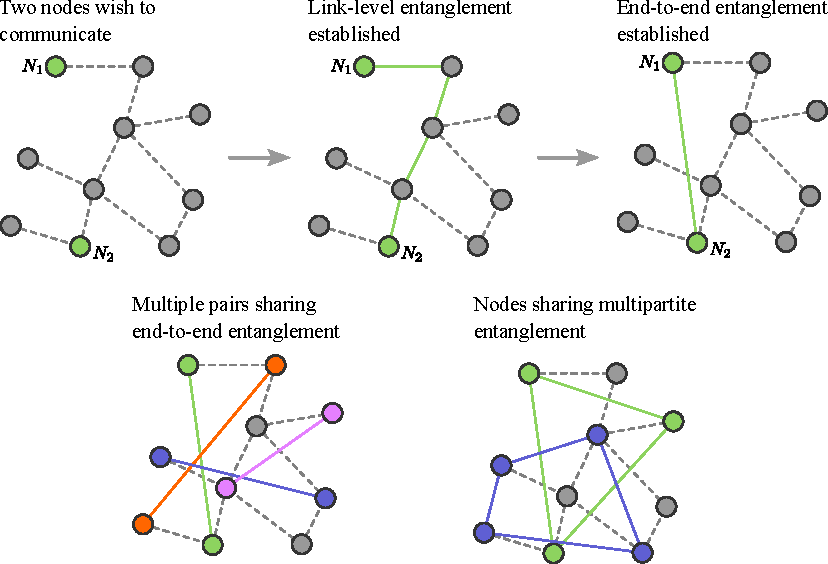
\includegraphics[width=\textwidth]{lesson14/14-1_bipartite_network.pdf}
    \caption[Bipartite and multipartite entanglement]{Bipartite and multipartite entanglement distribution in quantum networks.}
    \label{fig:14-1_bipartite_multipartite}
\end{figure}

One of the main jobs of a quantum network is to distribute entanglement.
Let's start by considering a concrete example.
Figure~\ref{fig:14-1_bipartite_multipartite} shows a quantum network.
The circles represent quantum nodes while the dashed lines represent physical links connecting neighboring quantum nodes.
Let's consider the scenario where Nodes $N_1$ and $N_2$ wish to establish shared entanglement in order to engage in quantum communication.
We saw in the previous chapter that in order to satisfy this request, the quantum network first creates link-level entanglement between neighboring nodes along the path connecting the nodes $N_1$ and $N_2$.
Entanglement swapping is then used to create a direct end-to-end bipartite entanglement between these nodes.
This example is rather constrained in the sense that it only shows two of the nodes trying to engage in quantum communication.
Well-designed quantum network should be able to accommodate multiple simultaneous requests for end-to-end entangled connections between multiple pairs of nodes as shown in Fig.~\ref{fig:14-1_bipartite_multipartite}. 

The quality of the distributed entanglement, whether bipartite or multipartite, matters greatly.
We saw that in entanglement-based QKD, the quality of the entanglement that is shared between Alice and Bob directly impacts the key that they are trying to establish.
If the entangled state shared by Alice and Bob is not perfect then the key that they are going to end up with after at the end of the protocol will also be only partially correlated.
This has two important consequences.
Firstly, it affects how well Alice and Bob can communicate.

More crucially, the quality of the entangled state affects the \textit{\textbf{security of the key}} that they can establish.
The entangled state may be imperfect due to natural noise introduced by the physical channels during the distribution process.
But it could also be a result of an eavesdropper Eve, trying to listen in on the secret communication between Alice and Bob as shown in Fig.~\ref{fig:14-1_QKD}.
If Alice and Bob want to maintain security of the information that they are wishing to communicate, they must assume that any imperfections in the entangled state have been introduced by Eve.
So the quality of the entangled state places an upper bound on the security of the key that can be established between Alice and Bob in the sense that \textit{\textbf{better quality of the entangled state implies stronger security}}.

We discussed in Section~\ref{sec:3-5_fidelity} that one way of quantifying the quality of an entangled state is the fidelity.
Given a ideal state \ket{\psi}, that the quantum network is trying to distribute, the fidelity of the actual mixed state $\rho$ shared between Alice and Bob is given by the expectation value of $\rho$ with respect to \ket{\psi},
\begin{equation}
    F \left( \rho, \ket{\psi} \right) = \bra{\psi}\rho\ket{\psi}.
\end{equation}
It is usually the case in quantum networks that the ideal state is one of the Bell pairs.
If the ideal state is \ket{\Phi^+}, then the fidelity if $F (\rho, \ket{\Phi^+}) = \bra{\Phi^+}\rho\ket{\Phi^+}$.
For noiseless quantum channels and operations, perfect quantum memories and in the absence of an eavesdropper, the distributed state will be the ideal state, $\rho = \ket{\Phi^+}\bra{\Phi^+}$.
The resulting fidelity is
\begin{equation}
    F \left( \rho, \ket{\Phi^+} \right) = \langle\Phi^+\ket{\Phi^+} \langle\Phi^+\ket{\Phi^+} = 1.
\end{equation}
On the other hand, the distributed state may some error, for example a Pauli $Z$ error on Bob's qubit.
This transforms the entangled state into an orthogonal Bell pair, $I \otimes Z \ket{\Phi^+} = \ket{\Phi^-}$, resulting in fidelity
\begin{equation}
    F \left( \rho, \ket{\Phi^+} \right) = \langle\Phi^+\ket{\Phi^-} \langle\Phi^-\ket{\Phi^+} = 0.
    \label{eq:14-1_fidelity_0}
\end{equation}
Typically, the distributed state will be mixed, and the fidelity will take values $ 0 \leq F(\rho, \ket{\Phi^+}) \leq 1$.

\begin{figure}[t]
    \centering
    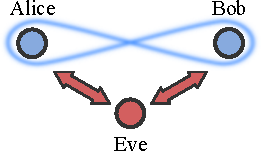
\includegraphics[width=0.4\textwidth]{lesson14/14-1_QKD.pdf}
    \caption[Eavesdropper Eve]{Eavesdropped Eve tampering with the distributed entangled state between Alice and Bob in order to gain information about the shared secret key.}
    \label{fig:14-1_QKD}
\end{figure}

Note that the lowest possible value of the fidelity does not imply that the distributed state is useless.
Far from it.
As we saw in Eq.~(\ref{eq:14-1_fidelity_0}), the fidelity vanishes when the distributed state is orthogonal to the ideal state \ket{\Phi^+}.
This means that the distributed state is also maximally entangled and can be used for quantum communication after an appropriate transformation.
For the case discussed in Eq.~(\ref{eq:14-1_fidelity_0}), the distributed state can be transformed into the ideal one by either Alice or Bob applying a local Pauli $Z$ operation,
\begin{align}
    \text{Alice applies } Z: \quad & Z \otimes I \ket{\Phi^-} = Z \otimes Z \ket{\Phi^+} = \ket{\Phi^+}, \\
    \text{Bob applies } Z: \quad & I \otimes Z \ket{\Phi^-} = I \otimes Z^2 \ket{\Phi^+} = \ket{\Phi^+}.
\end{align}
We used that fact that applying the Pauli $Z$ operation twice cancels its effect, $Z^2 = I$.

We saw that both extremes of the fidelity, $F(\rho,\ket{\psi}) = 1$ and $F(\rho,\ket{\psi}) = 0$, suggest that the distributed state is useful for quantum communication.
Does this mean that distributed states with intermediate values of fidelity are useful too?
Certainly not.
Let's consider a fully decohered state of two qubits given by the maximally mixed state,
\begin{equation}
    \rho = \frac{1}{4} \left( \ket{00}\bra{00} + \ket{01}\bra{01} + \ket{10}\bra{10} + \ket{11}\bra{11} \right).
\end{equation}
The fidelity of this state with respect to the ideal Bell pair \ket{\Phi^+} is
\begin{align}
    F \left( \rho, \ket{\Phi^+} \right) & = \frac{1}{4} \bra{\Phi^+} \left( \ket{00}\bra{00} + \ket{01}\bra{01} + \ket{10}\bra{10} + \ket{11}\bra{11} \right) \ket{\Phi^+} \nonumber\\
    & = \frac{1}{4} \left( \frac{1}{2} + \frac{1}{2} \right) = \frac{1}{4}.
\end{align}
We that it is $F=0.25$ that signifies the distributed state is ``completely useless''.

Fidelity is not the only useful metric when it comes to quantifying the quality of the distributed state.
The other method relies on the CHSH inequality which we saw plays a crucial role in the E-91 QKD protocol in Chapter~\ref{sec:10_E91}.
Named after its inventors Clauser, Horne, Shimony, and Holt, the CHSH inequality is a test of the quantumness of the correlations shared between Alice and Bob.
We saw that to test that Alice and Bob share the \ket{\Psi^+} Bell pair, they have to repeatedly measure in the following bases,
\begin{align}
    \text{Alice's measurement bases:}& & A_1 & = Z, & A_2 & = X \\
    \text{Bob's measurement bases:}& & B_1 & = \frac{Z - X}{\sqrt{2}}, & B_2 & = \frac{Z + X}{\sqrt{2}}.
\end{align}
Using the outcomes of the measurements, they can then compute the CHSH correlation,
\begin{equation}
    \mathcal{S} = \langle A_1 \otimes B_1\rangle + \langle A_1 \otimes B_2\rangle + \langle A_2 \otimes B_1\rangle - \langle A_2 \otimes B_2\rangle.
    \label{eq:14-1_CHSH_Psi_plus}
\end{equation}
For the ideal state, the expectation values can be computed according to $\langle A_i B_j \rangle = \bra{\Psi^+} A_i \otimes B_j \ket{\Psi^+}$, leading to the CHSH correlation of
\begin{equation}
    \left| \mathcal{S} \right| = 2\sqrt{2}.
\end{equation}
For the distributed state given by a mixed state $\rho$, the expectation values can be calculated via the more general expression $\langle A_i \otimes B_j \rangle = \text{Tr} \{ A_i \otimes B_j \rho \}$.
The distributed state is entangled provided that
\begin{equation}
    \left| \mathcal{S} \right| > 2.
\end{equation}
The CHSH inequality acts as a witness of entanglement, with $|\mathcal{S}| = 2$ being the critical threshold.
When Alice and Bob measure $|\mathcal{S}| > 2$, they know they share an entangled state.
On the other hand, when $|\mathcal{S}| < 2$, they cannot conclude anything. The distributed state could be entangled but it could be separable as well.
CHSH inequality violation is also directly linked to the security of the key that Alice and Bob can establish.
\textit{\textbf{Stronger violation of the CHSH inequality leads to more secure secret key.}}

What if the ideal state that Alice and Bob are trying to share some other Bell pair, let's say \ket{\Phi^+}.
Computing the CHSH violation in Eq.~(\ref{eq:14-1_CHSH_Psi_plus}) but computing the expectation values with respect to the new ideal state \ket{\Phi^+}, we get
\begin{align}
    \langle A_1 \otimes B_1 \rangle & = \frac{1}{\sqrt{2}} & \langle A_1 \otimes B_2 \rangle & = \frac{1}{\sqrt{2}} \\
    \langle A_2 \otimes B_1 \rangle & = - \frac{1}{\sqrt{2}} & \langle A_2 \otimes B_2 \rangle & = \frac{1}{\sqrt{2}}.
\end{align}
This leads to a vanishing CHSH correlation, $\mathcal{S} = 0$.
This is because the expression for the correlation in Eq.~(\ref{eq:14-1_CHSH_Psi_plus}) is not designed to witness entanglement when the ideal state is \ket{\Phi^+}.
We have encountered a similar situation when we computed the fidelity between two orthogonal Bell pairs.
Can we use a similar expression to Eq.~(\ref{eq:14-1_CHSH_Psi_plus}) that witnesses entanglement when the ideal state is \ket{\Phi^+}.
All we need to do is exchange the plus and minus signs in front of the last two terms,
\begin{equation}
    \mathcal{S} = \langle A_1 \otimes B_1\rangle + \langle A_1 \otimes B_2\rangle - \langle A_2 \otimes B_1\rangle + \langle A_2 \otimes B_2\rangle.
    \label{eq:14-1_CHSH_Phi_plus}
\end{equation}
Eq.~(\ref{eq:14-1_CHSH_Phi_plus}) yields $|\mathcal{S}| = 2\sqrt{2}$ when the expectation values are computed with respect to \ket{\Phi^+}.

We have seen that both the fidelity as well as the CHSH inequality offer suitable tools to quantify the quality of the distributed bipartite state.
We have to remember to take care when computing both quantities.
In order to obtain meaningful results, we need to use the correct ideal state in the case of fidelity, and the appropriate form of the correlation in the case of the CHSH inequality.




\section{Multipartite entanglement}
\label{sec:14-2_multipartite}

We have seen how quantum networks can establish bipartite entanglement between two of its nodes.
We may wish to distribute entanglement shared between more than two nodes as shown in Fig.~\ref{fig:14-1_bipartite_multipartite}.
Sometimes three clients may wish to engage in a quantum communication protocol that might require all of them to share a tripartite entangled state.
Any entangled state of more than two subsystems is called a \textit{\textbf{entangled multipartite state}}\index{multipartite entanglement}.
It is the job a quantum network to distribute multipartite entangled states between any disjoint subsets of nodes that ask for them.

We begin by considering entangled states of three qubits.
We saw that there are 4 possible computational basis, \ket{00}, \ket{01}, \ket{10}, and \ket{11}.
How many computational basis states are there in this case?
Now there are 8 such states,
\begin{align}
    \ket{000}, \; \ket{001}, \; \ket{010}, \; \ket{011}, \; \ket{100}, \; \ket{101}, \; \ket{110}, \; \ket{111}.
\end{align}
Any general three-qubit state can be expanded as a superposition of these computational basis states,
\begin{align}
    \ket{\psi} & = c_0\ket{000} + c_1\ket{001} + c_2\ket{010} + c_3\ket{011} \nonumber\\
    & + c_4\ket{100} + c_5\ket{101} + c_6\ket{110} + c_7\ket{111}.
\end{align}
often this superposition is written in a compact form as
\begin{equation}
    \ket{\psi} = \sum_{i=0}^7 c_i \ket{i},
\end{equation}
where the notation means that the ``$i$'' in \ket{i} is the binary number corresponding to the index in the coefficients $c_i$.
Depending on the values of the coefficients, we obtain different states, some of which will be entangled.

Let's look at a few examples of important entangled multipartite states.
The first state is one of the simplest but also one of the most important.
It is an equal superposition of \ket{000} and \ket{111}, and is known as the \textit{\textbf{GHZ state}}\index{GHZ state}, named after Greenberger, Horne, and Zeilinger,
\begin{equation}
    \ket{GHZ} = \frac{1}{\sqrt{2}} \left( \ket{000} + \ket{111} \right).
\end{equation}
Let's see what are some of the properties of the GHZ state.
A good start is to measure one of the qubits and see what the state of the remaining qubits is.
Consider measuring the first qubit in the Pauli $Z$ basis.
The projectors corresponding to the +1 and -1 outcomes are
\begin{align}
    \Pi^Z_+ & = \ket{0}\bra{0} \otimes I \otimes I, \\
    \Pi^Z_- & = \ket{1}\bra{1} \otimes I \otimes I,
\end{align}
respectively.
The probability of the measurement outcome being +1 is
\begin{align}
    \text{Prob} \{+1\} & = \text{Tr} \{ \Pi^Z_+ \ket{GHZ}\bra{GHZ} \} \nonumber\\
    & = \bra{GHZ} \left( \ket{0}\bra{0} \otimes I \otimes I \right) \ket{GHZ} \nonumber\\
    & = \frac{1}{2} \left( \bra{000} + \bra{111} \right) \left( \ket{0}\bra{0} \otimes I \otimes I \right) \left( \ket{000} + \ket{111} \right) \nonumber\\
     & = \frac{1}{2} \bra{000} \left( \ket{0}\bra{0} \otimes I \otimes I \right) \ket{000} \nonumber\\
     & = \frac{1}{2}.
\end{align}
Similarly, the probability of the measurement outcome being -1 is
\begin{equation}
    \text{Prob}\{-1\} = \text{Tr}\{\Pi^Z_-\ket{GHZ}\bra{GHZ}\} = \frac{1}{2}.
\end{equation}
If the measurement outcome is +1, the post-measurement state is
\begin{align}
    \frac{1}{\sqrt{\text{Prob}\{+1\}}} \Pi^Z_+ \ket{GHZ} & = \sqrt{2} \left( \ket{0}\bra{0} \otimes I \otimes I \right) \frac{1}{\sqrt{2}} \left( \ket{000} + \ket{111} \right) \nonumber\\
    & = \left( \ket{0}\bra{0} \otimes I \otimes I \right) \ket{000} \nonumber\\
    & = \ket{000}.
\end{align}
We see that the post-measurement state is correlated, all qubits are in the same state, but it is no longer entangled.
Measurement of a single qubit in the Pauli $Z$ basis is enough to destroy the entanglement shared between all three qubits.
This is also the case if the measurement outcome is -1,
\begin{equation}
    \frac{1}{\sqrt{\text{Prob}\{-1\}}} \Pi^Z_- \ket{GHZ} = \ket{111}.
\end{equation}

The next example of an entangled state of three qubits is called the \textit{\textbf{W state}}\index{W state}.
In the computational basis, it is a superposition of three terms,
\begin{equation}
    \ket{W} = \frac{1}{\sqrt{3}} \left( \ket{001} + \ket{010} + \ket{100} \right).
\end{equation}
We can again measure the first qubit in the computational basis again.
this time, the probabilities of the two possible outcomes are
\begin{align}
    \text{Prob}\{+1\} & = \text{Tr} \{ \Pi^Z_+ \ket{W}\bra{W} \} = \frac{2}{3}, \\
    \text{Prob}\{-1\} & = \text{Tr} \{ \Pi^Z_- \ket{W}\bra{W} \} = \frac{1}{3}.
\end{align}
This time the probabilities of the two outcomes are different from each other, unlike in the case of the GHZ state.
What is more interesting though are the post-measurement states corresponding to the outcomes of the measurement,
\begin{align}
    \text{outcome +1:} & \quad \ket{0}\ket{\Psi^+}, \label{eq:14-2_W_post_meas_0} \\
    \text{outcome +1:} & \quad \ket{1}\ket{00},
\end{align}
We see that when the outcome of the measurement is +1, the state of the remaining two qubits is a maximally entangled Bell pair.
This is in stark contrast to the GHZ state, where a single measurement destroys all entanglement regardless of the outcome.
This points at a fundamental difference between the GHZ state and the W state in terms of their entanglement properties.

This difference goes even deeper.
We can consider what happens to the entanglement if one of the qubits is lost.
Losing a single qubit of a GHZ state will completely destroy the entanglement.
On the other hand, a loss of a single qubit from a W state leaves the remaining two qubits entangled, albeit not maximally.
The W state is more robust to qubit loss than the GHZ state.

\begin{figure}[t]
    \centering
    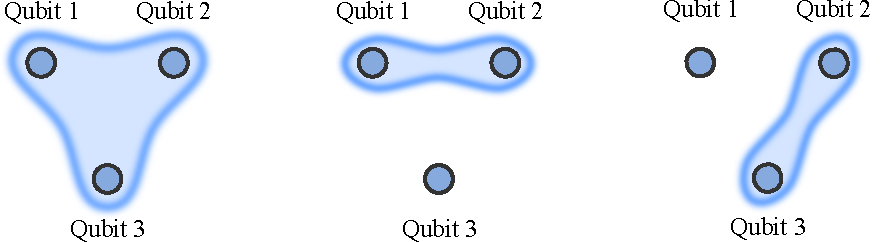
\includegraphics[width=\textwidth]{lesson14/14-2_monogamy.pdf}
    \caption[Monogamy of entanglement.]{Monogamy of entanglement restricts how three qubits can be correlated.}
    \label{fig:14-2_monogamy}
\end{figure}

Before moving onto $n$-partite entangled states, we will pause and think how the entanglement is shared between the three qubits.
There is a fundamental tradeoff to how strongly each pair of the qubits can be correlated, known as \textit{\textbf{monogamy of entanglement}}\index{monogamy of entnaglement}.
It states that the strength of entanglement between a pair of qubits places an upper bound on the amount of entanglement that the third qubit can share with either of the first two qubits.
Left panel of Figure~\ref{fig:14-2_monogamy} shows a general entnagled state of three qubits, where all three qubits are entangled with each other.
Examples corresponding to this situation are the GHZ and W states.
If a pair of qubits is in a maximally entangled state, for example \ket{\Phi+}, then monogamy of entanglement tell us that the third qubit must in a separable state with the first pair.
Total state of the three qubits can be written as
\begin{equation}
    \ket{\Phi^+}\ket{\psi},
\end{equation}
where \ket{\psi} is a pure state of the third qubit.
This is portrayed by the middle panel in Fig.~\ref{fig:14-2_monogamy}.
Similarly, if qubits 2 and 3 are maximally entangled like in the right panel of Fig.~\ref{fig:14-2_monogamy}, then the first qubit must be completely disentangled with either of them.
An example of this situation is given by hte post-measurement state of Eq.~(\ref{eq:14-2_W_post_meas_0}), where we measured the first qubit of a W state in Pauli $Z$ basis and obtained the +1 outcome.

Monogamy of entanglement is one of the most fundamental properties of quantum mechanics. It is unlike anything that exists in classical physics, and is one of the cornerstones and building blocks which we use in quantum technologies, and particularly in quantum communication.
Monogamy of entanglement is instrumental in guaranteeing security in the E91 QKD protocol.
The stronger Alice's and Bob's qubits are entangled the less information an eavesdroper can learn about the secret key.
If the shared pair of qubits between and Alice and Bob is maximally entangled, the eavesdropper can learn nothing.

We can extend our discussion of GHZ and W states to $N$ qubits.
The $N$-qubit GHZ state has the following form,
\begin{equation}
    \ket{GHZ} = \frac{1}{\sqrt{2}} ( \underbrace{\ket{00\ldots0}}_{N\text{ zeroes}} + \underbrace{\ket{11\ldots1}}_{N \text{ ones}} ).
\end{equation}
Notice that the normalization factor has not changed, even though this is now a GHZ state of $N$ qubits.
The W state can be extended to arbitrary number of qubits as well,
\begin{equation}
    \ket{W} = \frac{1}{\sqrt{N}} ( \underbrace{\ket{00\ldots01} + \ket{00\ldots10} + \ldots \ket{10\ldots00}}_{N \text{ terms}} )
\end{equation}
Since the $N$-qubit W state is an equal superposition of $N$ terms, he normalization factor is $1 / \sqrt{N}$.

\begin{figure}[t]
    \centering
    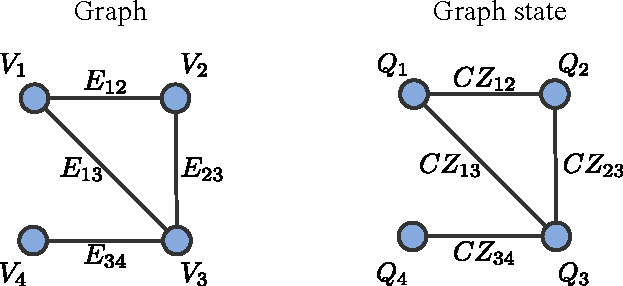
\includegraphics[width=0.6\textwidth]{lesson14/14-2_graph_state.pdf}
    \caption[Graph state.]{Graph state of four qubits and its underlying graph.}
    \label{fig:14-2_graph_state}
\end{figure}

GHZ and W states are not the only important examples of multipartite entangled states.
A prominent example of $N$-partite example is the \textbf{\textit{graph state}}\index{graph state}.
This state can be represented visually as a set of vertices $V$ which are connected by a set of vertices $E$.
Such an object is known as a \textit{\textbf{graph}}\index{graph}\footnote{Not to be confused with a graph of a function.}
Figure~\ref{fig:14-2_graph_state} shows an example of a graph with vertex set $V=\{V_1, V_2, V_3, V_4\}$, connected by edges from the edge set $E=\{ E_{12}, E_{23}. E_{13}, E_{34} \}$.
The corresponding graph state is obtained by placing a qubit at each vertex of the graph, initialized in $\ket{+} = (\ket{0} + \ket{1}) / \sqrt{2}$, and applying the \textbf{\textit{control-phase gate}}\index{control-phase gate} $CZ_{ij}$ between qubits whose vertices are connected by and edge $E_{ij}$.
The control-pahse gate $CZ$ is a two-qubit gate defined as
\begin{equation}
    CZ_{ij} = \ket{0}\bra{0}_i \otimes I_j + \ket{1}\bra{1}_i \otimes Z_j = \begin{pmatrix}
        1 & 0 & 0 & 0 \\
        0 & 1 & 0 & 0 \\
        0 & 0 & 1 & 0 \\
        0 & 0 & 0 & -1
    \end{pmatrix}.
\end{equation}
\begin{figure}[t]
    \centering
    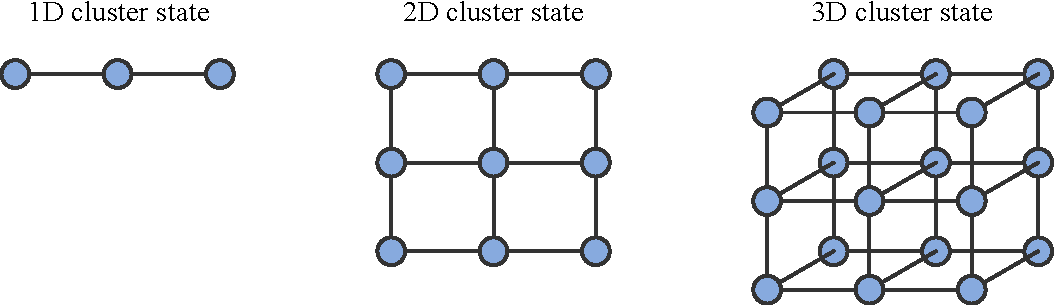
\includegraphics[width=\textwidth]{lesson14/14-2_cluster_state.pdf}
    \caption[Cluster state.]{Cluster states in different spatial dimensions.}
    \label{fig:14-2_cluster_state}
\end{figure}
The control-phase gate does nothing to the target qubit $j$ if the control qubit $i$ is in the \ket{0} state.
If the control $i$ is in the \ket{1}, the control-phase gate applies Pauli $Z$ to the target qubit $j$.
Applying this rule we can find the state vector for the graph state \ket{G} in Fig.~\ref{fig:14-2_graph_state},
\begin{align}
    \ket{G} & = CZ_{12} CZ_{23} CZ_{13} CZ_{34} |++++\rangle_{1234} \nonumber\\
    & = \frac{1}{4} ( |0000\rangle + |0001\rangle + |0010\rangle - |0011\rangle \nonumber\\
    & \; \; \; \; + |0100\rangle + |0101\rangle - |0110\rangle + |0111\rangle \\
    & \; \; \; \; + |1000\rangle + |1001\rangle - |1010\rangle + |1011\rangle \\
    & \; \; \; \; - |1100\rangle - |1101\rangle - |1110\rangle + |1111\rangle \\
    & = \frac{1}{2} ( |0+0+\rangle + |0-1-\rangle + |1-0+\rangle - |1+1-\rangle ).
\end{align}
If the underlying graph has a regular structure the resulting graph state is usually called a \textbf{\textit{cluster state}}\index{cluster states}.

Graph states and cluster states play an important role in quantum computation and quantum communication.
Cluster states are a resource state for a particular computational model known as ``measurement-based quantum computation''.
Graph states are useful in quantum error-correction as well as in many protocols in quantum communication.





\section{Clock synchronization}
\label{sec:14-3_clock_sync}

So we have seen in this module, the applications of how we can use entanglement. We saw the example of teleportation, and we saw the example of entanglement-based QKD. Here in the remaining two steps of this chapter, we will consider a few other examples of applying entanglement. And here in step three, we will look at clock synchronization. So before we say how we can synchronize clocks, let's ask the question- why we want to synchronize clocks. Well, establishing universal time standard is fundamentally important in many areas of modern life. The telecommunications networks require synchronized clocks, global positioning system (GPS), financial markets, transportation networks, these are all just a few examples of crucial importance to modern way of living. For example, if we look at the GPS, how it works, how it calculates the very accurate position of where we are, is it computes the distances to four satellites and then from that it can locate with very high degree of accuracy where we are placed on Earth. And in order to calculate this distance- is this R1, R2, R3, and R4, accurate timing is very important because even tiny errors in timing can result in huge positional errors. So how can we synchronize clocks? Well, there are really two classical methods and one quantum method which we will mention. The first one is due to Einstein. Imagine that we have two clocks- one is in possession of Alice and the other one is in possession of Bob, and they are trying to synchronize- Alice is trying to synchronize her clock with Bob's clock. So what she can do, is she can fire a pulse of light towards Bob. So the light is traveling to Bob and it reaches Bob. As soon as it reaches his clock, it bounces back and as it's doing that it sets Bob's clock ticking. Alice is measuring the time that it takes for the photon- for the light pulse to travel from her to Bob and bounce back. From that, she knows she can estimate the distance to Bob, she calculate the distance to Bob, and also she will know what's the round-trip time, and also what's the time in order for the photon to reach from Bob to Alice. Therefore, she knows how she can set her clock, and this will synchronize the two clocks together. However, in this scheme, Alice needs to know where Bob is located in order to correctly synchronize their clocks. A different scheme is for Alice to have some other smaller clock which she synchronizes locally with her clock, and then the small clock is very slowly, in fact adiabatically slowly, transferred to Bob where he receives the clock and then he can locally synchronize his clock with this received clock. And this scheme has to be done adiabatically slowly because of theory of relativity. Now the third scheme is realizing that qubits can act as tiny clocks. How does that work? Well qubits, they evolve in time. For example, if we prepare a qubit in an equal superposition of zero and one, we can make it change its state in time such that it goes around this x-y plane in the Bloch sphere with angular frequency "capital omega". So, it starts, we can initialize it in the state plus, and after some time capital T which is the period of precession, it completes one full circle. So it goes around an angle of two pi radians. So the period of precession is given by two pi divided by the angular frequency of precession. So, really in this sense, it's the same as a grandfather clock. If we can track how many times it goes around the x-y plane, we can track time knowing the angular frequency of precession. So the question now is- how can we synchronize two qubits? Let's say Alice has qubit one that is processing at a frequency capital omega, and Bob also has one that's also processing at the same frequency but this time there is some offset so it's lagging behind Alice's qubit clock. So this "delta" is quantifying the lag between- in terms of the angle between the point that's on the Bloch sphere in the x-y plane for Bob and for Alice, and what we are trying to do is we are trying to eliminate this offset delta in order for their clocks to be synchronized and show exactly the same time. So where is the main problem? Well, the problem is that Alice has her local time frame and Bob has his own local time frame, and somehow they need to communicate, like, say "my time frame is this, what is your time frame?", and they have to exchange messages in order to agree on a global time frame.

In fact, what they can do is they can do that by sharing entangled pairs of qubits. They can use these qubits to establish a global time frame.

So in that sense, entanglement is used as a global resource, and we have seen the similar scenario also in the entanglement-based QKD. There, we use entanglement and classical communication to correlate to- in order to establish a correlated secret key between Alice and Bob. That was the E91 protocol. In clock synchronization of qubits, we are using the global correlations that are present in a maximally entangled state in order to establish a global time frame and correlate these two qubit clocks together, therefore synchronizing them.

And quantum networks are instrumental in distributing bipartite entanglement, therefore allowing the various nodes in the network to synchronize their clocks and establish a global time frame.



\section{Distributed and blind quantum computation}
\label{sec:14-4_distributed_bqc}

Step Four: Distributed and Blind Quantum Computation

This will be our final example of the application of entanglement and quantum network in this chapter.

So let's talk about distributed quantum computation first. There is no reason for Alice to perform all of her quantum computation locally. Let's say that her resources are limited. Maybe she doesn't have the large number of qubits, or the qubits that she has are not of sufficient quality. But that doesn't mean that she cannot perform her quantum computation. What she can do is she can contact her friends, Bob, Charlie, Dave and Eve, who are also in possession of some limited computational resources. They also have some small quantum computers. And together, they can coordinate their resources and perform a larger quantum computation compared to if Alice did it only locally.

So here, Alice, Bob, Charlie, Dave and Eve, they all share some number- small number of qubits, and they can entangle in some them in some way, and also they can exchange quantum information by using the quantum network, or they can also exchange some entangled qubits, they can connect those local cluster states together in some larger cluster states and then perform computation on that. And there are many questions of interest, such as what is the most efficient way of networking the quantum processors together, how many messages do they need to exchange in order to coordinate their computational efforts, and also issues like trust- how can Alice trust. Maybe she doesn't trust all of the parties involved in the quantum computation. What does she need to do? How can quantum network help her in this situation?

Also, here we are assuming that she has some quantum resources. What if her quantum resources are extremely limited? So what do we mean by "extremely limited"? Let's say that she cannot do anything. She doesn't have a quantum computer but she would still like to delegate her quantum computation, and for simplicity let's just assume that Bob has a full-fledged, very powerful, large quantum computer where he can perform any quantum computation that he wishes or that Alice would ask him to do. So in this scenario, what she can just do is she can send him a classical message composed of many bits, describing to Bob exactly what computation she wishes him to perform. So, she needs to describe the input of the computation, the computation itself, and then Bob will just take this information and carry out the computation, and then tell Alice the output- the result of the computation. But in the process, what happens is he learns everything there is to know about the computation. He learns the input, he learns the computation itself, and he learns the output. Now, what if Alice doesn't want Bob to learn some of this information, or any of this information? Maybe she's trying to gain a competitive edge by performing some simulation of a molecule or a new material, and she doesn't want Bob to find it out because it's a trade secret. Can she still do something in this case? Well, she can if she's allowed to have some quantum resources. And particularly, we assume that Alice has the ability to generate single qubit states. So, what she can do is she generates these states and then she can randomly rotate them. Then she takes these keywords and she sends those to Bob, so she's using a quantum channel to communicate with Bob. But these qubits are not entangled, they're really just a bunch of single qubit states randomly rotated.

And then she sends him classical instructions about the computation. So she directs Bob- "take qubit one, perform this operation, take qubit two, perform that operation, take these two qubits and entangle them using this gate", and so on.

And in this way, Bob can perform whatever she is instructing him to do and then just return the final outcome. He communicates either in quantum way or classically to Alice about the result of the computation, and in this way Bob does not know the random rotations because those are still kept secret by Alice. So this prevents him from learning anything about the input, anything about the computation itself, and also anything about the output. He's basically doing this computation blind. He's performing some operations according to Alice's instructions, but because he doesn't know the initial states of the keywords, he doesn't really know what these operations mean. He cannot interpret them, therefore whatever he gets, he just performs the operations blindly, he gets some output, but he cannot interpret this output, he just returns it to Alice. The only thing that he can learn is the upper limit to Alice's computation. For example, if she sends him four qubits then he knows that she, Alice, could not have performed any computation that requires more than four qubits.



\newpage
\begin{exercises}
\exer{Let's look at measuring the W state in more detail.
Consider the projectors $\Pi_{\pm 1}^Z$ in Tab.~\ref{tab:3-2_projectors}.  To extend the measurement operators to measuring a subset of qubits, we need to tensor the projection operators with the identity matrix. 
\subexer{First, consider measuring a single qubit in the W state.
Calculate the probabilities of finding the $+1$ and $-1$ results using
$$\text{Pr} \{\pm 1\} = \langle W | \Pi_{\pm 1}^Z \otimes I \otimes I | W \rangle$$.}
\subexer{Calculate the probabilities of finding the $+1$ and $-1$ results when measuring in the X basis.
}
\subexer{Calculate the probabilities of finding the $+1$ and $-1$ results when measuring in the Y basis.
}
}

\exer{Now consider measuring two of the three qubits in the W state. You will need for projectors instead of just two.

\subexer{Calculate the probabilities of finding the $(+1,+1)$, $(+1,-1)$, $(-1,+1)$ and $(-1,-1)$ results when measuring in the Z basis.
}

\subexer{Calculate the probabilities of finding the $(+1,+1)$, $(+1,-1)$, $(-1,+1)$ and $(-1,-1)$ results when measuring in the X basis.
}

\subexer{Calculate the probabilities of finding the $(+1,+1)$, $(+1,-1)$, $(-1,+1)$ and $(-1,-1)$ results when measuring in the Y basis.
}

}


\end{exercises}

